%-------------------------------------------------------------------
% Document class and package definitions
%-------------------------------------------------------------------
\documentclass[12pt,a4paper,openright,final,twoside,ieeetran]{main}



%Included for Gather Purpose only:
%input "thesisreferences.bib"

\begin{document}

\defaultbibliography{thesisreferences.bib}     %% Change this only.
\defaultbibliographystyle{unsrt}        %% Could be changed if you like 
                                           %% references typeset differently.
%-------------------------------------------------------------------
% Define title, author, etc.
%-------------------------------------------------------------------
\def\thesistitle{Embedded IoT System for Eclipse Arrowhead}
\def\theauthor{Albin Martinsson}
\def\theaddress{Dept.\ of Computer Science and Electrical Engineering\\
Lule{\aa} University of Technology\\ Lule{\aa}, Sweden}

\def\supervisors{Jan van Deventer}
\def\supervisorstring{Supervisor:} % Edit here if you have only one supervisor
\def\dedication{To my dad Bengt-Göran Martinsson, a special thanks for proof reading is required...}

% Read abstract and preface from separate files.
% Make sure these exist. See example files.
\def\theabstract{The abstract is a mini thesis on its own. It should contain the briefest of motivation and problem description, what has been done, and summarize the results. The purpose is to give the reader a quick view of the content, and encourage the reader to read the rest of the thesis. It's also helpful to put the reader in the right frame of mind for the rest of the thesis. This section is typically anything between one paragraph for short research papers (of 8 pages) to a page for a full thesis}
\def\thepreface{The research conducted in this thesis has been funded by the Arrowhead Tools project.
}


% Change here if you want to remove the logo printed on the first page

\def\thelogo{\includegraphics[width=\textwidth]{example-image-a} \\ \vspace{1cm}} % old EU logo
%\def\thelogo{} % no logo

% The definitions above could be put directly in the function call below,
% but is here defined explicitly, for the purpose of clarity.

\startpreamble
  {\thesistitle}
  {\theauthor}
  {\theaddress}
  {\supervisors}
  {\dedication}
  {\theabstract}
  {\thepreface}
  {\thelogo}

%%%%%%%%%%%%%%%%%%%%%%%%%%%%%%%%%%%%%%%%%%%%%%%%%%%%%%%%%%%%%%%%%%%%
%% Begin Part I
%%%%%%%%%%%%%%%%%%%%%%%%%%%%%%%%%%%%%%%%%%%%%%%%%%%%%%%%%%%%%%%%%%%%


%% Initialize part containing the thesis introduction chapters
\startchapters
\begin{bibunit}
%------------------------ Start chapter 1 --------------------------
% The \makechapter command takes three arguments
%  1) An abbreviated version of the chapter name,
%     to be used as page header
%  2) String to be added to the table of contents
%  3) The chapter name, possibly split in to lines,
%     as in Chapter 2 below.
%
%  The different arguments can have different line breaks.
%
% The actual contents of the chapter is included by removing the
% comment from the \input line below. Make sure the file
% chapter1.tex exists.
%-------------------------------------------------------------------

\makechapter{Introduction}{Introduction}{Introduction\label{ch1}}
\pagenumbering{arabic}
\section{Background}
The number of devices connected to the Internet has risen from 7 billions in 2018 to an estimated 35 billions in 2021 according to Security Today and that number is only going to increase.[1] %https://securitytoday.com/Articles/2020/01/13/The-IoT-Rundown-for-2020.aspx?Page=2%. 
\section{Motivation}
With the numbers of devices connected to the Internet, IOT-devices from now on, rising to an estimated 38.6 billion devices world wide by 2025 the need to enable communication between those devices have never been bigger.
\section{Problem definition}
This project aims to investigate the possibilities, benefits and 
limitations of using Arrowhead Framework on embedded devices
in contrast to commercially available solutions such 
as Amazons Amazon Web Services, AWS 
from now on, and Microsofts Azure.  
The way to measure the difference between either 
using a central broker, the MQTT protocol used by AWS and Azure or using peer to peer, 
HTTP protocol used by the Arrowhead framework to handle the communication between devices in terms of latency, 
energy consumption and
security.

\section{Equality and ethics}
Equality and ethics are learning objectives for the program and should be reflected upon in the thesis if applicable. This section can be omitted if not at all relevant to the problem definition, but in many cases the thesis topic touches upon these topics even if it is outside the scope of the work itself and in such cases a single paragraph may be sufficient to cover the reflection.
\section{Sustainability}
Similar to the equality and ethics section this is one of the learning objectives for the program and should be reflected upon in the thesis if applicable. For a quick overview of what is considered to be included in sustainability you can see the united nations list of sustainability goals: https://www.un.org/sustainabledevelopment/sustainable-development-goals/
\section{Delimitations}
Describe what is not covered in the thesis. Things you realize may have to be addressed to create a complete solution, but that would be too much work, or that may simply be out of the scope of your scientific area.
\section{Thesis structure}
Describe how the rest of your thesis is organized. (e.g. In section 2 we discuss, in section 3 there is a... etc.). This is really just to help guide the reader to where different parts of your work can be found.


\makechapter{Related work}{Related work}{Related work\label{ch2}}
\section{Internet of things}
Cluster of European research projects regarding the Internet of Things:
\begin{quote}
    'Things' are active participants in buissness, information and social processes where they are enabled to interact and communicate aming themselves and with the enviorment by exhchanging data and information sensed about the envoirment while reacting autonomously to real/physical world events and influencing it by runnign processes that trigger actions and create services with or without direct human intervention.\cite{Gubbi2013}
%Fix correct qoute on this!
\end{quote} 

Gubbi et. al. defines the Internet of Things as:
\begin{quote}
    Interconnection of sensing and actuating devices providing the ability to share inforamtion across platforms through a unified framework, developing a common operating picture for enabling innovative applications. 
    This is achieved by seamless large scale sensing, data analytics and information representation using cutting egde ubiquitous sensing and cloud computing.\cite{Gubbi2013}
\end{quote}

\section{Industry 4.0}
%Industry 4.0 definition.
Lasi argues that the term industry 4.0 was coined beforehand as a planned fourth industrial revolution.\cite{Lasi2014}
The use of internet of things devices, IoT devices from now on, and cyber-physical systems, CPS from now on is what defines the fourth industrial revolution Vadiya means.\cite{Vaidya2018}
See figure x for a short historic overview of previous industrial revolutions.   
\begin{figure}
    \centering
    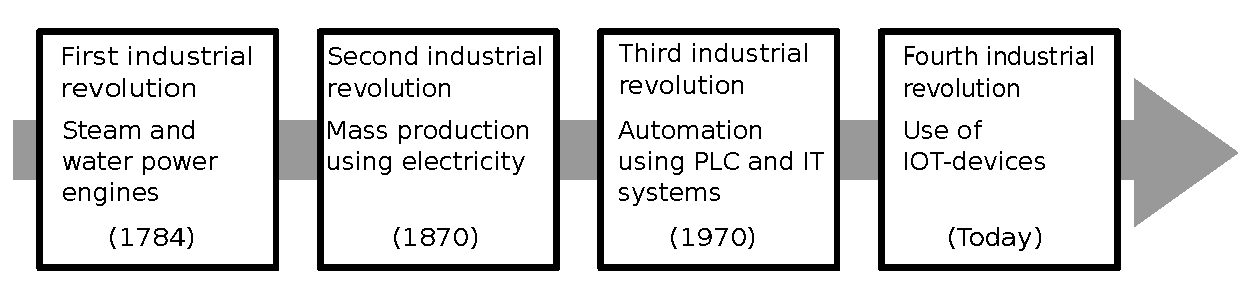
\includegraphics[width=\textwidth]{Pictures/Industrial_revolution.pdf} 
    \caption{Historic overview of previous industrial revolutions}
    \label{Indutrial revolutions}
\end{figure}

According to Vadiya industry 4.0 promotes the connection of sensors and devices both to the internet and to other sensors or devices.\cite{Vaidya2018} 

%Intelligent  sensors.
Hozdić states that a sensor is a device capable of providing an appropriate output in response to a measured value.\cite{Hozdic2015}
One key feature of an intelligent sensor is that to increase the level of information processing it processes the information at a logical level Hozdić argues.\cite{Hozdic2015}
An Intelligent sensor  is capable of executing actions based on the measured value in contrast to regular sensors, making them easier to set up and use means Hozdić.\cite{Hozdic2015} 

%Cyber Physical Systems (CPS).
Hozdić defines a cyber-physical system, CPS, as a new generation of a system that integrates both physical and computer abilities.\cite{Hozdic2015}
A cyber-physical system consists of two parts, one cybernetic and one physical.
The cybernetic part of the system can be viewed as a summation of logic and sensor units while the physical part of the system can be viewed as a summation of the actuator units Hozdić adds.\cite{Hozdic2015}
Xu et. al. states that cyber-physical systems are a key part of Industry 4.0. In contrast to the simple embedded systems of today will be exceeded due to advances in CPS that enable enhanced capability, scalability, adaptability, resiliency, safety, usability, and security.\cite{Xu2018}
Hozdić argues that the CPS can share and receive information from intelligent sensors that connect to digital networks is what enables and form an internet of things.\cite{Hozdic2015}
 
\section{Arrowhead framework}
%Local cloud.
A local cloud is defined as a self-contained network with at least the three mandatory systems deployed, more on those in a later paragraph. 
Delsing et.al. also argues that the three mandatory core systems running a local cloud also need at least one application system deployed.\cite{Delsing2017}

%Service and systems.
Two terms have to be introduced to further understand what the Eclipse Arrowhead framework aims to accomplish, services and systems.
Delsing et. al. defines a system as what is providing or consuming a service.\cite{Delsing2017} 
Furthermore, a service is defined as what is used to convey information between a provider and a consumer Delsing et. al. argues.\cite{Delsing2017}

%Mandatory core systems.
The Eclipse Arrowhead framework, Arrowhead from now on, consists of three mandatory core systems according to Delsing et. al.\cite{Delsing2017}
To fully operate a local cloud as defined in the previous section it must, according to Delsing, contain:
\begin{itemize}
    \item Service registry system.
    \item Authorization system. 
    \item Orchestration system.\cite{Delsing2017}
\end{itemize} 

%Service registry system.
The service registry system is responsibly for enabling discovery and registring services Delsing et. al. states.\cite{Delsing2017} 
According to the Eclipse Arrowhead projects own GitHub page the service registry system provides the database which stores the offered services in the local cloud.\cite{Github2021}
The Github page also states the three main objectives of the service registry system are:
\begin{itemize}
    \item To allow the application system to register available services to the database. 
    \item Remove or update available services from the database.
    \item Allow application system to use the lookup functionality of the registry.
\end{itemize}
%Authorization system.
The Authorization system contains two databases for keeping track of which system can consume services from which other systems, depending on whether or not the Application system are in the same cloud or not according to the projects Github page.\cite{Github2021}
The GitHub documentation also states that if the authorization happens within the same cloud it is called intra-cloud authorization and if it happens across two local clouds it is called inter-cloud authorization.\cite{Github2021}
%Orchestrator system.
The Orchestration system is responsible for pairing and finding service providers and consumers Delsing et. al. declares.\cite{Delsing2017} 
Delsing et. al. continues to state that the orchestrator also stores the orchestration requirements and the resulting orchestration rules.\cite{Delsing2017} 
The project's documentation argues that the main objective of the orchestrator system is to find an appropriate provider for the requesting consumer system.\cite{Github2021}
The documentation also states that there are two types of orchestration, store orchestration, and dynamic orchestration.
Store orchestration uses the database orchestration store to find predefined orchestration rules.
Dynamic orchestration on the other hand searches the entire local cloud, or even other clouds, to find the matching provider.\cite{Github2021}

\section{Security}
%Introduction.
Meneghello et. al. argues that the increasing number of IoT devices and the pervasive nature of new smart home or healthcare devices can pose a real threat to the users' integrity.
Sensitive information Meneghello et. al. defines as a video recording of the user's home, the user's location, access to buildings, health monitoring, and industrial processes.\cite{Meneghello2019}

%Secruity challenges.
Meneghello et. al. states the security requirements of an IoT system can be divided into three different operational levels, namely the information, access, and functional level.\cite{Meneghello2019}
The information level should guarantee that the integrity, anonymity, confidentiality, and privacy of the system are preserved. 
Meaning that messages should not be altered during transmission, the identity of the data source and the clients' private information remains hidden and that data cannot be read by third parties Meneghello et. al. argues.\cite{Meneghello2019} 
The access level provides a guarantee that only legitimate users are allowed access to the network and the devices associated with that network. 
It also guarantees that users within the network only use resources they are allowed to use Meneghello et. al. states.\cite{Meneghello2019}
The functional level should guarantee the continued functionality of a network even in the case of malfunction or a malicious attack Meneghello et. al. adds.\cite{Meneghello2019}

%Pricacy.
Zhang also argues that privacy is a big concern with IoT devices and suggests two solutions data collection policy and data anonymization.\cite{Zhang2014}
A policy that describes how the data is collected from the devices would restrict the flow of data, therefore ensuring privacy preservation can be ensured Zhang states.\cite{Zhang2014}
Data anonymization means that the private information sent by the IoT devices is either encrypted or that the relation of the data and its owner is concealed according to Zhang.\cite{Zhang2014}

%Encryption.
Meneghello et. al. argues that one of the main aspects of security within IoT is to ensure that the data sent is the data received and that the data has not been tampered with or read during transmission.
The most important operation to guarantee that is the use of encryption, which converts the message sent in plain text to an encrypted message only readable with a decryption key Meneghello et. al. states.\cite{Meneghello2019}
Meneghello et. al. states that there are two mechanisms for encryption, symmetric and asymetric.\cite{Meneghello2019} 
Symmetric encryption is when the same key is used for encryption and decryption, so it has to be shared with both the sender and receiver.
Asymmetric encryption on the other hand only shares the public key and the sender and receiver have their own private keys Meneghello et. al. means.\cite{Meneghello2019}

%End-to-End encryption.
Hassija et. al. states the importance of end-to-end encryption and the challenges it poses for IoT systems.\cite{Hassija2019}
End-to-end encryption is required to ensure the confidentiality of the data, the application should not let anyone except the intended recipient read the messages sent Hassija adds.\cite{Hassija2019}

%Authentification.
Noor, Meneghello, and Zhang state the importance of authentification in IoT systems.\cite{Noor2019,Meneghello2019,Zhang2014} 
Noor adds that 60\% of all IoT systems use authentification to grant access to the user.\cite{Noor2019}  
Zhang argues that public key cryptosystem provides more security compared to symmetric encryption schemes, but has the drawback of having high computational overhead.\cite{Zhang2014} 

%Lightweight cryptography.
Noor argues that conventional cryptographic primitive is unsuitable for IoT devices due to their lack of computational power and limited battery life and memory capacity.\cite{Noor2019}
With IoT devices lacking capabilities as background Noor, Meneghello, and Zhang all agree that a push for lightweight cryptography is required to ensure the security of these devices.\cite {Noor2019,Meneghello2019,Zhang2014} 

\section{Communication} 
%MQTT
MQTT, Message Queue Telemetry Transport, is a lightweight messaging invented by IBM suitable for IoT Wukkadada means.\cite{Wukkadada2018} 
MQTT is a publish/subscribe protocol that requires a minimal footprint and bandwidth to connect an IoT device according to HIVEMQ.\cite{MQTT2021}
MQTT consists of an MQTT broker and MQTT clients, where the broker is responsible for sending messages between the sender and its recipients.\cite{Wukkadada2018}
A client on the other hand publishes a message to the broker that other clients can subscribe to HIVEMQ adds.\cite{MQTT2021}

%HTTP/HTTPS
HTTP, HyperText Transfer Protocol, is a request/response protocol consisting of clients and servers that communicate by exchanging individual messages. 
The clients are responsible for the requests and the servers are responsible for the response Mozilla developer network clarifies. \cite{HTTP2021} 
In contrast to the lightweight MQTT protocol with low overhead and bandwidth, HTTP can cause serious bandwidth issues Wukkadada adds. \cite{Wukkadada2018}
The biggest benefits to using HTTP are that it supports the RESTful Web architecture and that it is a globally accepted web messaging standard Naik suggests. \cite{Naik2017} 

%Comparisson 
Naik argues that HTTP exceeds MQTT in message size, message overload, power consumption, resource requirements, bandwidth, and latency. 
All things that are considered negative for a protocol.\cite{Naik2017}
On the other hand, HTTP exceeds MQTT in interoperability, standardization, security, and provisioning Naik adds.\cite{Naik2017}
All things that are considered positive for a protocol.
Shariatzadeh argues that that HTTP may be expansive for many IoT devices but it can be beneficial due to the interoperability since it is developed for the web originally.\cite{Shariatzadeh2016}
Wukkadada also points out the lower power consumption of the MQTT protocol but adds that the more verbose HTTP protocol can be easier for developers to understand.\cite{Wukkadada2018}
Wukkada drives home the point of choosing MQTT for IoT devices.\cite{Wukkadada2018}

\makechapter{Theory}{Theory}{Theory\label{ch3}}
\section{Theory}
%SWAGGER


%AHF

%MYSQL
%ARM MBED
%MBED-HTTP

\makechapter{Implementation}{Implementation}{Implementation\label{ch4}}
\section{Implementation}
%overview
The system consists of three major parts, the consumer on the stm32 board, a Python flask app as a provider, and the arrowhead framework.
The main objective of the arrowhead framework is to connect the consumer and the provider in a safe and structured way.
The consumer is built with C/C++ using ARMs' mbed os, and mainly the mbed-http library. 

\subsection{System architecture}

\subsection{System component}


\makechapter{Evaluation}{Evaluation}{Evaluation \label{ch5}}
\section{Evaluation}
Describe the test setup to verify that your problems from 1.3 have been solved. This can be done in different ways depending on focus of your problems. Some problems may purely objective, such as "improve the performance of X compared to Y". These are easy to evaluate since you simply need to compare the performance, and perhaps compare against a few more technologies that you have listed in Section 2 (related work). In other cases the problems may be very subjective, such as "Create a mobile app that can be used while driving, and which shows the most fuel efficient time to change gear". This problem will require a user-study in which several persons drive without the application, you calculate the fuel consumption, then they drive with the application and then you calculate the fuel consumption again. Then you collect the objective measurements (fuel consumption comparisons) and the subjective opinions from the users about whether the application was unobtrusive, usable, etc. (typically via a questionnaire)

\makechapter{Discussion}{Discussion}{Discussion\label{ch6}}
This thesis aimed to investigate whether it was possible to use an embedded device in conjunction with the Eclipse Arrowhead framework.
If that was possible, this thesis also aimed to show the advantages and limitations of using the Eclipse Arrowhead framework on embedded devices.
Another goal of this thesis was to show that using the Arrowhead framework on embedded devices provides a ready-to-make example for people to try out the framework.
To fill a void in the Arrowhead project GitHub with a complete example ready to compile and using an online compiler.

\section{Choice of development environment}
The IDE, integrated development environment, chosen for this thesis stood between the Mbeb online compiler and the STM CUBE IDE. 
The STM cube IDE requires setup on the local machine, installing C and Cmake, but provides shorter compilation time.
The Mbed online compiler requires no setup on the local machine but takes much longer to save and compile the code.

Both compilation time and an easy setup are favorable attributes for an IDE, and it all depends on the end goal.
If the goal were to try out multiple different iterations of the same source code, then STM cube IDE would be the best choice.
On the other hand, if the goal was to provide an example of a framework or concept and get the users started as quickly and painless as possible, the Mbed online compiler is the obvious choice.
The latter fitted the goals of this thesis better and was therefore chosen. 

Both IDEs provide ready to run example that features different aspects of the development boards, and both contain an example of connecting the board to the internet.
The Mbed online compiler, in conjunction with arm Mbed OS, provides an easy and intuitive way to get started on desired projects.
The Mbed online compiler has its drawbacks as well. 
When using it, the user is pushed into using libraries integrated into the Mbed OS 6.
It is possible to use outside libraries but more often than not, resulting in a rabbit hole of including header files.
On the other hand, STM Cube IDE works similarly to a local C-program. 
If the header files are in the include folder or installed locally, they can be used without much effort.

The STM Cude IDE also supports code generation from Cube MX, letting the user choose which peripherals to be included and adding initiation code before developing a project.
Cube MX also supports importing supported libraries, generating the required include folders and header files for the user beforehand. 
When using the Mbed online compiler, all the peripherals, sensors, and libraries have to be initialized by the user.
It will result in a trade-off between ease of use, performance, and customizability.

One disadvantage of using the STM cube IDE is that all applications will become platform-dependent.
STM cube IDE requires the user to have a Windows computer. 
Mbed online compiler, on the other hand, builds everything in the browser.
When the build is done, the Mbed online compiler prompts the user to download a .bin file that can be dragged to the STM32 B-L4S5I-IOT01A board, as if storing a file on a flash drive.
The STM32 B-L4S5I-IOT01A board compiles the .bin file and outputs the result to the user, no need to install Cmake or other toolchains. 

\section{Provider arcitechture}
The implementation in this thesis follows the publish/subscribe model, as described in the related work section. 
The STM32 B-L4S5I-IOT01A board is the publisher, and the remote computer will act as the subscriber.
The board has to find where to send the temperature data and sends it in predefined intervals after that. 
The implementation made in this thesis lacks the functionality of acting as a server, serving a request from a consumer.


In the Eclipse Arrowhead system, a provider system will typically be passive, reacting to requests.
When speaking of it in an HTTP sense, the provider will act as a server.
A consumer will usually act as a client and find the provider's address to request services from the provider. 
In this implementation, the provider will find the consumer's address and send the temperature information.
The service it provides is sending the reading from the temperature sensor in specific time intervals. 
It is important not to get hanged upon the terminology as both a provider and a consumer are considered systems in the Eclipse Arrowhead framework. 
In essence, they are the same thing and can be used interchangeably.
It all depends on how the service is defined.

Depending on the application, it might be more efficient to send the data when the consumer demands it. 
It is possible to imagine the opposite as well.
If a system relies on past information, it might be more efficient to send the data at a specified rate.
If the system has to process the data and perhaps depends on a lot of data, it may be more efficient to use the subscribe/publish model. 
Negating the need for the embedded device to respond to requests can increase energy efficiency by having it boot at specific times to send the data.
If a system relies on real-time data creating a REST API to handle these requests would be the next logical step for developing this example. 
This will be covered in the future work section in the next chapter.

\section{Comparing different frameworks}
The previous chapters showed that it was possible to use the Eclipse Arrowhead framework with embedded devices. It also showed the advantages of using the framework.
The main advantage was the response time, having on average 17.5 times faster response time than its competitors. 
A faster response time could be a great advantage when dealing with real-time applications when a fast response is as essential as a correct one. 

One disadvantage of using the Eclipse Arrowhead could be the lack of supported hardware.
This thesis was the first example to show that it was possible to connect to the arrowhead framework on embedded devices.
In contrast, Amazon Web Services have many examples of using different hardware. 
Amazon Web Services also has examples showcasing the different sensors and connection possibilities of their supported boards.
Creating an open-source example of using the Eclipse Arrowhead framework could inspire others to start developing embedded Arrowhead applications, expanding the functionality of this implementation.

The eclipse Arrowhead Framework requires hardware to run on, a service that has to be paid for with Amazon Web Services. 
It is probably cheaper to purchase hardware and run the Eclipse Arrowhead on a larger scale, but that requires an upfront cost.
In smaller-scale applications or when trying out a proof of concept, the prices offered by Amazon Web Services are hard to beat.
When using Amazon Web Services, the user relies on that their hardware and network runs continuously, an issue which magnitude showed its face this fall. 

One significant advantage of using Amazon Web Services is its services offered out of the box.
Lambda functions, S3 buckets, and all the functionality that follows with them is something the user will have to implement on their own if choosing the Eclipse Arrowhead framework.
On the other hand, if the user wants to do something not supported by Amazon Web Services, they will be constrained.
As with the choice of IDE, it will result in a trade-off between ease of use and customizability.

Another significant advantage of Amazon Web Services is the support for and enforcement of using HTTPS.
When deploying a 'Thing' to the AWS IoT Core, a certificate is generated and has to be included in the source code.
The security issues raised in the related work section illustrate the need for HTTPS and other security measures for IoT devices in production.
When developing a proof of concept, as this thesis has been doing, the requirement of HTTPS might be overstated.
It becomes a trade-off between usability, development time, and security. 
If the intent is to demonstrate that the Eclipse Arrowhead framework works on embedded devices, the use of HTTPS and all the extra steps for implementing that might do more harm than good. 

The Eclipse Arrowhead framework supports HTTPS and encourages its users to use it.
There is documentation for generating Arrowhead compliant certificates and support for it in the Java implementation of a client.
However, it proved to be challenging to implement and beyond the scope of this thesis. 
The attempts of implementing HTTPS will be covered more in the future work section in the next chapter.

\makechapter{Conclusions and future work}{Conclusions and future work}{Conclusions and future work\label{ch7}}
This chapter summarizes the thesis by outlining its accomplishments and remaining work left to do.
Section 7.1 contains the conclusion, and in section 7.2 the reader can find a description of work to be done in the future.
\section{Conclusion}
This thesis examines the possibility of using an Eclipse Arrowhead framework local cloud on an embedded device, namely the STM32 B-L4S5I-IOT01A board. 
It was possible to implement functionality for the Eclipse Arrowhead framework on the STM32 B-L4S5I-IOT01A board, having the board send temperature readings to a computer within a local network.

Another goal of this thesis was to provide an easy-to-run example of the Eclipse Arrowhead framework that anyone could compile by anyone wanting to give the framework a try, a missing feature right now for embedded devices.
The implementation was done with usability in mind, making it easy for users to try the code.
The desired usability was achieved with the Mbed online compiler's code importation and minimum setup development environment, allowing users to try out the Eclipse Arrowhead framework on the STM32 B-L4S5I-IOT01A board.

The thesis also examines the benefits of using the Eclipse Arrowhead framework compared to its competitors Amazon Web Services and Microsoft Azure.
The thesis showed some benefits in terms of response time when running a local cloud instead of using a remote service such as Amazon Web Services. 
A 17.5 decrease in average response time was recorded.
Maximum and minimum response times decreased by 1.9 and 134 times, respectively.  

\section{Future work}
%Intro.
The research presented in this thesis can take many different directions moving forward.
Two main issues were raised during this thesis, security and having the STM32 B-L4S5I-IOT01A board act as a server.
The following sections will address these two issues.
\subsection{Security}
%Security.
We have to address the security issues raised in the previous chapters if the implementation done in this thesis ever is to be used by the industry in production. 
This thesis made several attempts at implementing HTTPS; the Mbed-HTTP library has support for HTTPS, and STM cube IDE has support for wolfSSL. 

The problem to be solved before implementing HTTPS is how the Eclipse Arrowhead framework handles certificates in programming languages other than Java.
Both Mbed and STM cube has examples using HTTPS that works, and getting started with Amazon Web Services uses HTTPS with a user-generated certificate.
One of the main issues is that the certificates are self-signed, meaning no trusted certificate authority has signed them. 
The self-signed certificates proved to be the main obstacle for implementing HTTPS using C. None of the libraries, Mbed-HTTP or wolfSSL, could trust the certificate from the Eclipse Arrowhead framework.
There is a need to conduct further research using the certificates generated by the Eclipse Arrowhead framework on embedded devices.
One area of research could be to move away from the .pk12 format, generally used by java applications, and include more support for the .pem format used by C and many other languages.
Another area of research needed is lightweight cryptography and possible ways to move away from the idea that an IoT device has its certificate.
A concept that quickly becomes unbearable when dealing with thousands of devices in one network.

\subsection{Server implementation}
%Server implementation.
Before being appliable to the industry, one would have to solve the board's inability to react to requests. 
The issue of reacting to requests is of utmost importance. 
Both the Mbed online compiler and the STM Cube IDE have a working example of an HTTP server that can request the temperature data from a generated webpage.
Those examples use pure HTTP requests and responses, leading to very lengthy and challenging messages to parse. 
Future research that promotes the same usability as Mbed-HTTP and responding to the request would greatly benefit the Eclipse Arrowhead framework.  

A server implementation on the STM32 B-L4S5I-IOT01A board could also have great educational potential by using it in courses for young adults or aspiring engineers.
With the number of IoT devices connecting to the internet only increasing, understanding connected embedded devices is crucial for future engineers. 
Introducing concepts like IoT and embedded system programming early in an engineering degree and real-life examples could enhance knowledge and spike interest for those subjects, making aspiring engineers ready for the future.


\makechapter{References}{References}{References\label{ch8}}
\def\bibname{}
\putbib


\makebib
\end{bibunit}

\end{document}
